%% -*- coding: utf-8; -*-

\documentclass[
  master
  brazilian
]{ThesisPUC}


%%%
%%% Additional Packages
%%%

  \usepackage[brazilian]{babel}      %% in ThesisPUC.cls
  %% \usepackage[utf8]{inputenc}        %% .
  %% \usepackage[T1]{fontenc}           %% .
  %% \usepackage{lmodern}               %% .
  %% \usepackage[pdftex]{graphicx}	%% .

  \usepackage{tabularx}
  \usepackage{multirow}
  \usepackage{multicol}
  \usepackage{colortbl}
  \usepackage[%
    dvipsnames,
    svgnames,
    x11names,
    fixpdftex
  ]{xcolor}
  \usepackage{numprint}
  \usepackage{textcomp}
  \usepackage{booktabs}
  \usepackage{amsmath}
  \usepackage{enumitem}
  \usepackage{amssymb}
  \usepackage{textcomp}
% \usepackage{etoolbox}

%% numprint 
\npthousandsep{.}
\npdecimalsign{,}

%% ThesisPUC option
%\tablesmode{figtab} %% [nada, fig, tab ou figtab]
%\abreviationsmode{none} %% [none ou use] %% Default is [use]


%%%
%%% Counters
%%%

%% uncomment and change for other depth values
%% \setcounter{tocdepth}{3}
%% \setcounter{lofdepth}{3}
%% \setcounter{lotdepth}{3}
%% \setcounter{secnumdepth}{3}


%%%
%%% New commands and other global definitions
%%%

% -*- coding: iso-8859-1; -*-

%%%
%%% Newcommands
%%%

\newcommand{\degree}{\ensuremath{^\circ}}

\newcommand{\cetem}{Centro de Tecnologia Mineral}

\newcommand{\mybulletOB}{%
  % \textbullet
  % \checkmark
  $\triangleright$
  %\textopenbullet
}

\newcolumntype{L}{>{\raggedright \arraybackslash}X}
\newcolumntype{R}{>{\raggedleft \arraybackslash}X}
\newcolumntype{C}{>{\centering \arraybackslash}X}
\newcolumntype{M}[1]{>{\centering\hspace{0pt}}m{#1}}

\newcommand{\mrcel}[2]{%
\begin{tabular}[c]{@{}c@{}}#1\\#2\end{tabular}}

\newcommand{\mrcell}[2]{%
\begin{tabular}[l]{@{}l@{}}#1\\#2\end{tabular}}

\newcommand{\mrcelthree}[3]{%
\begin{tabular}[c]{@{}c@{}c@{}}#1\\#2\\#3\end{tabular}}

\newcommand{\mrcelcolorg}[2]{%
\begin{tabular}{l}\rowcolor{Gainsboro}#1\\#2\end{tabular}}

\newcommand{\mytbcimg}[3]{%
  \multicolumn{1}{C}{\parbox[c]{#1}{\includegraphics[width=#2]{#3}}}}


%%%
%%% Misc.
%%%

\usecolour{true}

%%%
%%% Titulos
%%%

\author{Vinicius da Silva Costa Almada}
\authorR{Almada, Vinicius da Silva Costa}

\advisor{Luiz Fernando Martha}{Prof. Dr.}
\advisorR{Martha, Luiz Fernando}
% If the advisor's department is different from author's department, uncomment the next line and type the correct name and acronym of advisor's institution.
%\advisorInst{institution name}{acronym}

\coadvisor{André Luís Müller}{Dr.}
\coadvisorR{Müller, André Luís}
\coadvisorInst{Instituto Tecgraf/PUC-Rio}{Tecgraf/PUC-Rio}

%% \title{Desenvolvimento de um sistema de microscopia digital para
%%  classificação automática de tipos de hematita em minério de ferro}

\title{Modelagem Topológica e Geométrica de Processos aplicados a multi-seções Geológicas}

\titleuk{Topological and Geometric Modeling of Processes applied to Geological multi-sections}

%% \subtitulo{Aqui vai o subtitulo caso precise}

\day{31}
\month{Julho}
\year{2021}

\city{Rio de Janeiro}
\CDD{XYZ.AB}
\program{Engenharia Civil}
\school{Centro Técnico Científico}
\university{Pontifícia Universidade Católica do Rio de Janeiro}
\uni{PUC-Rio}

%%%
%%% Jury
%%%

\jury{%
  \jurymember{Banca Um}{Prof.}
    {Universidade Federal de Minas Gerais}{UFMG}
  \jurymember{Banca Dois}{Prof.}
    {Universidade Federal de Ouro Preto}{UFOP}
  \jurymember{Banca Três}{Dr.}
    {Centro de Tecnologia Mineral}{CETEM/MCTI}
  \jurymember{Banca Quatro}{Dr.}
    {Departamento de Engenharia Química e de Materiais}{PUC-Rio}
}

%%%
%%% Resume
%%%

\resume{%
  Bacharel em Engenharia Civil pelo Instituto Federal de Educação, Ciência e Tecnologia do Maranhão (IFMA), formou-se em 2018. Foi bolsista de programas de Iniciação Científica PIBITI – IFMA, com projeto de desenvolvimento de software para Mecânica dos Solos e um segundo na área de Dinâmica das Estruturas. Este último foi base para seu Trabalho de Conclusão de Curso, cujo objetivo foi desenvolver um software para análise dinâmica de estruturas sujeitas à carregamento sísmico. Desde o fim de 2019 atua no Instituto Tecgraf como bolsista no Grupo de Modelagem Geológica de Sistemas Petrolíferos}

%%%
%%% Acknowledgment (REMINDER TO SCHOLARSHIP STUDENTS. Do not forget to thank the agencies that supported your work.)
%%%

\acknowledgment{%
  \noindent Primeiro parágrafo de agradecimento ...
  \bigskip

  \noindent Segundo parágrafo de agradecimento ...
}

%%%
%%% Catalog prekeywords
%%%

\catalogprekeywords{%
  \catalogprekey{Engenharia Civil e Ambiental}%
  \catalogprekey{Engenharia}%
}

%%%
%%% Keywords
%%%

\keywords{%
  \key{Geologia Estrutural}
  \key{Restauração de Seções Geológicas}
  \key{Restauração de Superfícies Geológicas}
  \key{Estrutura de Dados}
}

\keywordsuk{%
  \key{Structural Geology}%
  \key{Restoration of Geological Sections}%
  \key{Restoration of Geological Surfaces}%
  \key{Data Structures}%
}

%%%
%%% Abstract
%%%

\abstract{%
  Esse projeto visa desenvolver, dentro do Sistema Recon MS, um fluxo de trabalho que envolve as áreas de geologia estrutural, estratigrafia e geologia de reservatórios. Esse fluxo inicia com a restauração de modelos geológicos (seções e superfícies). Dentro do Sistema Recon busca-se aprimorar as ferramentas em seu ambiente de visualização 3D, denominado multi-seções, ou MS. Através de duas formas diferentes serão desenvolvidas ferramentas que irão prover as geometrias para o ambiente de simulação estratigráfica (para cada tempo geológico): 1) mapeamento de litologias e outras propriedades durante a restauração de seções, que por sua vez gerarão os paleo-relevos; 2) restauração de superfícies em si, que elimina a necessidade do mapeamento do item 1. A importância de ambas as estratégias consiste no fato de que nem sempre é possível obter bons resultados com restauração de superfícies, já que os mecanismos de restauração de seções desenvolvidos são muito mais geológicos. Para o mapeamento é necessária a criação de uma estrutura de dados que represente a malha de superfícies com possibilidade de armazenar informações, como propriedades e ligações entre as entidades das superfícies com as seções. Atualmente o Sistema Recon trabalha de forma totalmente desacoplado entre a estruturas de dados que representa as seções geológicas e a estrutura que representa as superfícies geológicas (horizontes, falhas e tipo do sal). Já para a segunda abordagem, ou seja, a restauração de superfícies, prevê-se o desenvolvimento de um módulo computacional de otimização dedicada a eliminar os buracos das superfícies que estão sendo restauradas incluindo restrições de deslocamento, sobre as falhas geológicas, das sub-superfícies abaixo da superfície restaurada.
}

\abstractuk{%
  This project aims to develop, within the Recon MS System, a workflow that involves the areas of structural geology, stratigraphy and reservoir geology. This flow begins with the restoration of geological models (sections and surfaces). The Recon System seeks to improve the tools in its 3D visualization environment, called multi-sections, or MS. Through two different forms, tools will be developed that will provide the geometries for the stratigraphic simulation environment (for each geological time): 1) mapping of lithologies and other properties during the restoration of sections, which in turn will generate paleo-reliefs; 2) surface restoration itself, which eliminates the need for mapping item 1. The importance of both strategies is the fact that it is not always possible to obtain good results with surface restoration, since the section restoration mechanisms developed are much more geological. For mapping, it is necessary to create a data structure that represents the surface mesh with the possibility of storing information, such as properties and links between the entities of the surfaces and the sections. Currently the Recon System works in a totally decoupled way between the data structures that represent the geological sections and the structure that represents the geological surfaces (horizons, faults and salt type). For the second approach, that is, the restoration of surfaces, it is foreseen the development of a computational optimization module dedicated to eliminate the holes of the surfaces that are being restored including displacement restrictions, on the geological faults, of the sub-surfaces below the restored surface.}

%%%
%%% Dedication
%%%

\dedication{%
  Dedicado lorem ipsum
}

%%%
%%% Epigraph
%%%

\epigraph{%
  My beautifull epigraph
}
\epigraphauthor{Wassily Kandinsky}
\epigraphbook{Regards sur le passé}

%%%
%%% Hyphenation
%%%

\hyphenation{PON-TI-FÍ-CIA}

%%%
%%% 
%%%

\begin{document}

  % -*- coding: utf-8; -*-

\chapter{Linha de Mapeamento}

Um dos recursos presentes no Sistema Recon é a \textbf{linha de mapeamento}, cujo objetivo é auxiliar na interpretação dos resultados gerados na restauração do modelo. Essa linha armazena referências a pontos topológicos da malha da seção. Com isso, é possível ter uma linha que acompanha a movimentação da malha de um cenário a outro.

As linhas de mapeamento (Figura~\ref{fig-linemap}) permitem realizar um mapeamento geométrico ao longo de uma restauração tomando como base uma linha-guia poligonal definida em um dado cenário. Essa linha pode ser criada em qualquer cenário, mesmo em seções já restauradas.

\begin{figure} [h]
  \begin{center}
    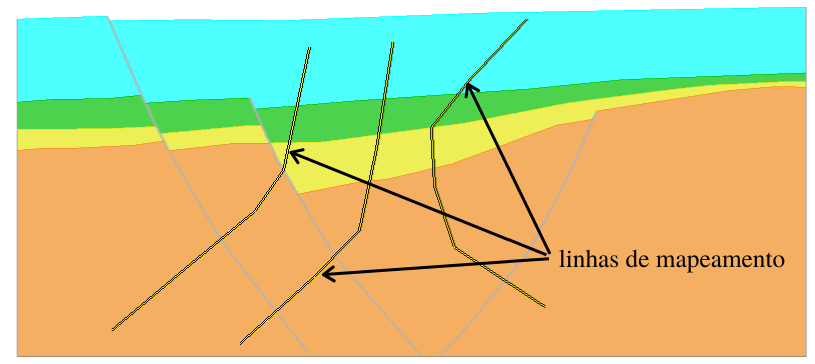
\includegraphics[width=400pt]{images/fig-linhas-de-mapeamento-ed}
    \caption{Linhas de mapeamento em uma seção.}\label{fig-linemap}
  \end{center}
\end{figure}

Cada face de uma seção tem como atributo uma malha triangulada, e as linhas de mapeamento são definidas no sistema de coordenadas local da malha de cada uma das faces. Além disso, é possível que uma linha de mapeamento cruze diversas malhas, por isso, a linha de mapeamento é definida como um conjunto de "partes" de linha de mapeamento, sendo cada parte pertencente a um trecho contínuo em uma mesma face. O processo de criação do mapeamento da linha é feito para cada parte. Na Figura~\ref{fig-linemap-malhas} é possível ver uma linha de mapeamento cortando algumas malhas diferentes.

\begin{figure} [h]
  \begin{center}
    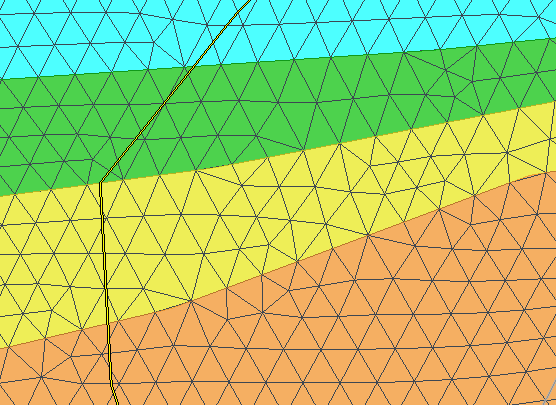
\includegraphics[width=350pt]{images/fig-linhas-de-mapeamento-malhas}
    \caption{Linhas de mapeamento cortando múltiplas faces.}\label{fig-linemap-malhas}
  \end{center}
\end{figure}

A primeira etapa desse mapeamento é a criação da linha-guia, a partir disso é feita a separação nas partes a serem processadas. É realizado um mapeamento com informações topológicas da interseção da parte com a malha. Essa ação consiste em fazer uma relação entre um ponto da parte da linha-guia e um ponto em uma entidade topológica da malha.

Por exemplo, na Figura~\ref{fig-linemap-parts} estão evidenciadas as partes que formam a linha de mapeamento. Cada uma dessas partes é representada pela entidade chamada \textit{LineMapPart}.

\begin{figure} [h]
  \begin{center}
    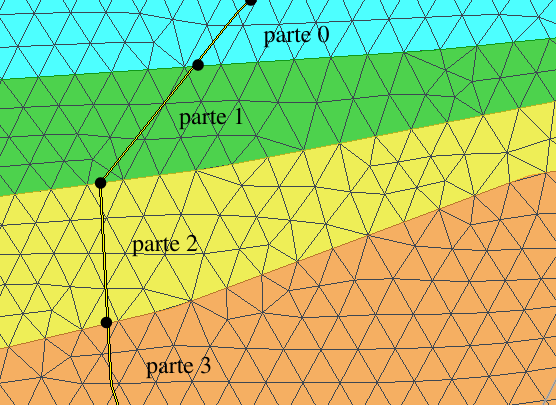
\includegraphics[width=350pt]{images/lm-parts}
    \caption{Partes de uma linha de mapeamento}\label{fig-linemap-parts}
  \end{center}
\end{figure}


  %% -*- coding: utf-8; -*-

\chapter{Review}

This is the second chapter...

In this chapter, let's have a nice table:

%% -*- coding: utf-8; -*-

\begin{table} [!h]
  \caption{Principais minerais de ferro e suas classes.\cite{29}}\label{tab:2-4}
  ~\\[-1mm]
   \begin{tabularx}
     {\textwidth}
     { p{2.0cm}
       p{2.5cm}
       p{3.3cm}
       p{1.3cm}
       p{2.7cm}}

     \textbf{Classes}
     & \textbf{Minerais}
     & \textbf{\mrcel {Fórmula}{Química}}
     & \textbf{\mrcel{Teor}{de Fe}}
     & \textbf{\mrcel{~~Designação}{~~Comum}}
     \\\toprule

     ~ \\[-6mm]
     \multirow{5}{*}{Óxidos}& Magnetita
     & $Fe_{3}O_{4}$
     & ~72,4
     & \mrcel{~~Óxido ferroso}{~~férrico}
     \\%\midrule

     & Hematita
     & $Fe_{2}O_{3}$
     & ~69,9
     & ~~Óxido férrico \\[2mm]

     & Goethita
     & $FeO(OH)$
     & ~62,8
     & \multirow{2}{*}{\mrcel{Óxido-hidróxido}{de ferro}} \\[2mm]


     & Lepidocrocita
     & $FeO(OH)$
     & ~62,8 &
     \\\midrule

     Carbonato
     & Siderita
     & $FeCO_{3}$
     & ~48,2
     & \mrcel{~~~~Carbonato}{~~~~de Ferro}
     \\\midrule

     \multirow{2}{*}{Sulfetos}
     & Pirita
     & $FeS_{2}$
     & ~46,5
     & \multirow{2}{*}{~} \\[2mm]


     & Pirrotita
     & $FeS$
     & ~63,6
     & ~
     \\\midrule

     \multirow{10}{*}{Silicatos}
     & Fayalita
     & $Fe^{2+}_{2}(SiO_{4})$
     & ~54,8
     & \mrcel{~~~~Grupo da}{~~~~Olivina} \\[4mm]

     & Laihunite
     & $Fe^{2+}Fe^{3+}_{2}(SiO_{4})_{2}$
     & ~47,6
     & \mrcel{~~~~Grupo da}{~~~~Olivina} \\[4mm]

     & Greenalita
     & \mrcell{$2Fe^{2+}_{2}6Fe^{3+}Si_{2}$}{$4O_{5}(OH)_{3,3}$}
     & ~44,1
     & \mrcel{~~~~Grupo da}{~~~~Serpentina} \\[4mm]

     & Grunerita
     & \mrcell{$Fe^{2+}_{7}(Si_{8}O_{22})$}{$(OH)_{2}$}
     & ~39,0
     & \mrcel{~~~~Grupo dos}{~~~~Anfibólios} \\[4mm]

     & Fé-antofilita
     & \mrcell{$Fe^{2+}_{7}(Si_{8}O_{22})$}{$(OH)_{2}$}
     & ~39,0
     & \mrcel{~~~~Grupo dos}{~~~~Anfibólios}
     \\\midrule
   \end{tabularx}
\end{table}

% -*- coding: utf-8; -*-

\newcommand{\coltworowone}{%
\begin{tabular}{ l @{\extracolsep{2mm}}X }
  \mybulletOB
    & Cristais ~~ muito	\\[-1.2mm]
  ~ & pequenos, 	\\[-.4mm]
  ~ & $<0.01$ mm. \\
  \mybulletOB & Textura porosa. \\
  \mybulletOB
    & Contatos pouco	\\[-1.2mm]
  ~ & desenvolvidos.
\end{tabular}}

\newcommand{\coltworowtwo}{%
\begin{tabular}{ l @{\extracolsep{2mm}}X }
  \mybulletOB
    & Cristais euédricos \\[-1.2mm]
  ~ & isolados ~ ou ~ em \\[-1.2mm]
  ~ & agregados. \\
  \mybulletOB
    & Cristais compac- \\[-1.2mm]
  ~ & tos.
\end{tabular}}

\newcommand{\coltworowthree}{%
\begin{tabular}{ l @{\extracolsep{2mm}}X }
  \mybulletOB
    & Hematita ~~ com \\[-1.2mm]
  ~ & hábito de magne- \\[-1.2mm]
  ~ & tita. \\
  \mybulletOB
    & Oxidação segundo \\[-1.2mm]
  ~ & os planos ~ crista- \\[-1.2mm]
  ~ & lográficos da mag- \\[-1.2mm]
  ~ & netita. \\
  \mybulletOB
    & Geralmente ~ po- \\[-1.6mm]
  ~ & rosa.
\end{tabular}}

\newcommand{\coltworowfour}{%
\begin{tabular}{ l @{\extracolsep{2mm}}X }
  \mybulletOB
    & Formatos irregu- \\[-1.2mm]
  ~ & lares ~~ inequidi- \\[-1.2mm]
  ~ & mensionais. \\
  \mybulletOB
    & Contatos irregula-\\[-1.2mm]
  ~ & res, ~ geralmente \\[-1.2mm]
  ~ & imbricados.
 \end{tabular}}

\newcommand{\coltworowfive}{%
\begin{tabular}{ l @{\extracolsep{2mm}}X }
  \mybulletOB
    & Formatos regula- \\[-1.2mm]
  ~ & res ~~ equidimen- \\[-1.2mm]
  ~ & sionais. \\
  \mybulletOB
    & Contatos ~~ retilí- \\[-1.2mm]
  ~ & neos ~ e ~ junções \\[-1.2mm]
  ~ & tríplices. \\
  \mybulletOB
    & Cristais compac-\\[-1.6mm]
  ~ & tos.
 \end{tabular}}

\newcommand{\coltworowsix}{%
\begin{tabular}{ l @{\extracolsep{2mm}}X }
  \mybulletOB
    & Cristais inequidi- \\[-1.2mm]
  ~ & mensionais, hábi- \\[-1.2mm]
  ~ & to tabular. \\
  \mybulletOB
    & Contato retilíneo. \\
  \mybulletOB
    & Cristais compac- \\[-1.6mm]
  ~ & tos.
 \end{tabular}}

\newcommand{\coltworowseven}{%
\begin{tabular}{ l @{\extracolsep{2mm}}X }
  \mybulletOB
    & Material cripto- \\[-1.2mm]
  ~ & cristalino.  \\
  \mybulletOB
    & Estrutura colofor- \\[-1.2mm]
  ~ & me, hábito botri- \\[-1.2mm]
  ~ & oidal.  \\
  \mybulletOB
    & Textura porosa.
 \end{tabular}}

\begin{table} [!p]
    \caption{Main morphologies of hematite.\cite{14}}\label{tab:2-5}
    ~\\[-2mm]
  \begin{tabularx}{\textwidth}{@{\extracolsep{0pt}}C @{\extracolsep{0pt}}C C C}

    \textbf{Tipo}
    & \textbf{Características}
    & \textbf{\mrcel{Forma}{Textura}}
    & \textbf{\mrcel{Ilustração}{Esquemática}}
    \\\toprule

    ~ \\[-6mm]
    \mrcel{Hematita}{Microcristalina}
    & \coltworowone
    & \mytbcimg{2.3cm}{2.9cm}{images/Microcristalina}
    & \mytbcimg{2.6cm}{2.5cm}{images/MicrocristalinaEsq}
    \\\midrule

    ~\\[-6mm]
    Magnetita
    & \coltworowtwo
    & \mytbcimg{2.3cm}{2.9cm}{images/Magnetita}
    & \mytbcimg{2.6cm}{2.9cm}{images/MagnetitaEsq}
    \\\midrule

    ~\\[-5mm]
    Martita
    & \coltworowthree
    & \mytbcimg{2.3cm}{2.9cm}{images/Martita}
    & \mytbcimg{2.6cm}{2.9cm}{images/MartitaEsq}
    \\\midrule

    ~\\[-5mm]
    \mrcel{Hematita}{Lobular}
    & \coltworowfour
    & \mytbcimg{2.3cm}{2.9cm}{images/Lobular}
    & \mytbcimg{2.6cm}{2.9cm}{images/LobularEsq}
    \\\midrule

    ~\\[-5mm]
    \mrcel{Hematita}{Granular}
    & \coltworowfive
    & \mytbcimg{2.3cm}{2.9cm}{images/Granular}
    & \mytbcimg{2.6cm}{2.9cm}{images/GranularEsq}
    \\\midrule

    ~\\[-5mm]
    \mrcel{Hematita}{Lamelar}
    & \coltworowsix
    & \mytbcimg{2.3cm}{2.9cm}{images/Lamelar}
    & \mytbcimg{2.6cm}{2.9cm}{images/LamelarEsq}
    \\\midrule

    ~\\[-5mm]
    \mrcelthree{Hidróxidos de}{ Fe (Goethita-}{Limonita)}
    & \coltworowseven
    & \mytbcimg{2.3cm}{2.9cm}{images/Goethita}
    & \mytbcimg{2.6cm}{2.9cm}{images/GoethitaEsq}
    \\\midrule

  \end{tabularx}
\end{table}


\section{Hematite}

A hematita é o mineral de ferro mais importante devido a sua alta
ocorrência em vários tipos de rochas e suas origens diversas.\cite{30}
A composição química deste mineral é Fe$_{2}$O$_{3}$, com uma fração
mássica em ferro de 69,9\% e uma fração mássica em oxigênio de
30,1\%.\cite{31}

...


\subsection{Martite}

A hematita é o mineral de ferro mais importante devido a sua alta
ocorrência em vários tipos de rochas e suas origens diversas.\cite{30}
A composição química deste mineral é Fe$_{2}$O$_{3}$, com uma fração
mássica em ferro de 69,9\% e uma fração mássica em oxigênio de
30,1\%.\cite{31}

...


\subsubsection{Globular}

A hematita é o mineral de ferro mais importante devido a sua alta
ocorrência em vários tipos de rochas e suas origens diversas.\cite{30}
A composição química deste mineral é Fe$_{2}$O$_{3}$, com uma fração
mássica em ferro de 69,9\% e uma fração mássica em oxigênio de
30,1\%.\cite{31}

...

\subsubsection{Escaping percent in a title:  100\%}

  %% -*- coding: utf-8; -*-

\chapter{Conclusão}

Assim, como uma proposta para trabalho futuro, pode-se buscar combinar
os dois enfoques...

  %% ...
  \arial
  \bibliography{tiny}
  \normalfont
  % -*- coding: utf-8; -*-

\appendix
\chapter{Published paper}

The following paper was published ...

\end{document}
